\documentclass[../AnalisiDeiRequisiti.tex]{subfiles}


\begin{document}
\section{Casi d'uso}
\subsection{Gerarchia degli attori}
\begin{figure}[!h]
    \centering
    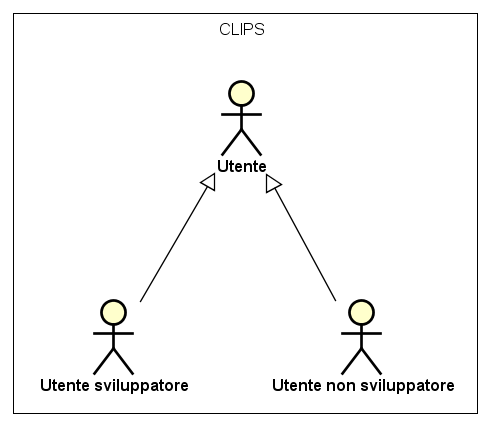
\includegraphics[scale=0.60]{img/diagramma_attori.png}
    \caption{Attori e relazioni tra essi}\label{fig:attori} 
\end{figure}
\hypertarget{UCG}{}
\subsection{Caso d'uso UCG: Utilizzo generale del prototipo}

        \begin{figure}[!h]
            \centering
            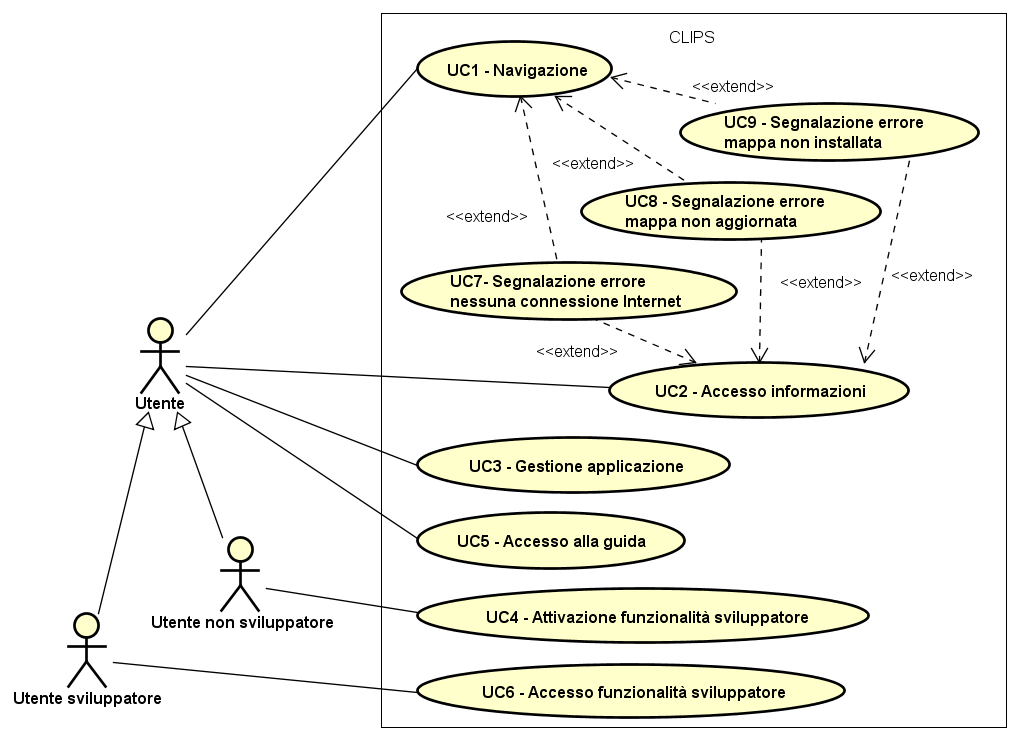
\includegraphics[scale=0.95, width=\textwidth]{img/UCG.png}
            \caption{Caso d'uso UCG: Utilizzo generale del prototipo}\label{fig:UCG} 
        \end{figure}
\begin{itemize}
\item \textbf{Attori}: utente;
\item \textbf{Descrizione}: un utente deve poter accedere alla navigazione, consultare informazioni relative all'edificio nel suo complesso o ad un singolo POI, modificare le impostazioni utente ed accedere alla guida dell'applicazione. Un utente non sviluppatore eredita tutti i casi d'uso di utente ed inoltre deve poter attivare le funzionalità avanzate dell'applicazione. Un utente sviluppatore, oltre ad ereditare tutti i casi d'uso di utente, deve poter accedere alle funzionalità avanzate dell'applicazione; 
      \item \textbf{Precondizione}: l'utente ha avviato l'applicazione installata nel proprio dispositivo;

        \item \textbf{Flusso principale degli eventi}:
          \begin{enumerate}
          \item L'utente può accedere alla navigazione (\hyperlink{UC1}{UC1});
          \item L'utente può accedere alle informazioni relative all'intero edificio o a singolo POI dell'edificio (\hyperlink{UC2}{UC2});
          \item L'utente può accedere alla gestione dell'applicazione (\hyperlink{UC3}{UC3});
          \item L'utente non sviluppatore può accedere alla sezione per lo sblocco delle finzionalità di sviluppatore (\hyperlink{UC4}{UC4});
          \item L'utente può accedere alla guida (\hyperlink{UC5}{UC5});
          \item Lo sviluppatore può accedere alle funzionalità avanzate (\hyperlink{UC6}{UC6});

      \end{enumerate}
    \item \textbf{Postcondizione}: il sistema ha erogato le funzionalità richieste dall'utente;
    \item \textbf{Scenari Alternativi}:
      	\begin{itemize}
    			\item Nel caso in cui l'utente voglia accedere alla navigazione di un edificio la cui mappa non risulti aggiornata o presente nel dispositivo:
    			\begin{enumerate}
    				\item Viene presentato un errore esplicativo (\hyperlink{UC7}{UC7}).
    			\end{enumerate}
          \item Nel caso in cui l'utente voglia accedere alle informazioni di un edificio la cui mappa non risulti aggiornata o presente nel dispositivo:
          \begin{enumerate}
            \item Viene presentato un errore esplicativo (\hyperlink{UC7}{UC7}).
          \end{enumerate}
      	\end{itemize}
  \end{itemize}
\hypertarget{UC1}{}
\subsection{Caso d'uso UC1: Navigazione}

        \begin{figure}[!h]
            \centering
            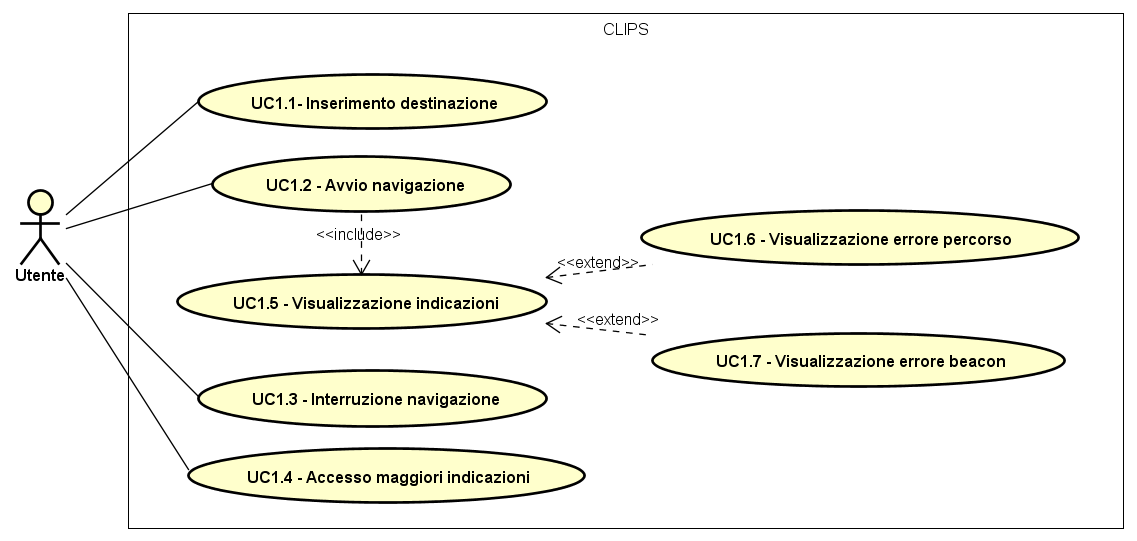
\includegraphics[scale=0.95, width=\textwidth]{img/UC1.png}
            \caption{Caso d'uso UC1: Navigazione}\label{fig:UC1} 
        \end{figure}
\begin{itemize}
\item \textbf{Attori}: utente;
\item \textbf{Descrizione}: l'utente deve poter essere guidato dal sistema verso una destinazione scelta. Quando l'utente si trova in navigazione deve poter: interrompere la navigazione in corso, accedere ad indicazioni più dettagliate; 
      \item \textbf{Precondizione}: l'utente si trova nella sezione dedicata alla navigazione, ha attivato il Bluetooth, si trova all'interno di un edificio mappato ed il dispositivo deve rilevare almeno un beacon;

        \item \textbf{Flusso principale degli eventi}:
          \begin{enumerate}
          \item L'utente indica il POI che vuole raggiungere (\hyperlink{UC1.1}{UC1.1});
          \item L'utente avvia la navigazione verso il POI scelto (\hyperlink{UC1.2}{UC1.2});
          \item L'utente può interrompere la navigazione in corso  (\hyperlink{UC1.3}{UC1.3});
          \item L'utente può accedere ad indicazioni più dettagliate  (\hyperlink{UC1.4}{UC1.4});

      \end{enumerate}
	\item \textbf{Postcondizione}: l'utente ha raggiunto la destinazione scelta oppure ha interrotto la navigazione;
    \item \textbf{Scenari Alternativi}:
    	\begin{itemize}
      		\item Nel caso in cui l'utente segua un percorso diverso da quello consigliato:
      		\begin{enumerate}
         		\item Viene presentato un errore esplicativo (\hyperlink{UC1.6}{UC1.6});
      		\end{enumerate}
      		\item Nel caso in cui l'utente si trovi in un area non coperta da beacon:
      		\begin{enumerate}
         		\item Viene presentato un errore esplicativo (\hyperlink{UC1.7}{UC1.7}).
      		\end{enumerate}
      	\end{itemize}

  \end{itemize}
\hypertarget{UC1.1}{}
\subsection{Caso d'uso UC1.1: Inserimento destinazione}

        \begin{figure}[!h]
            \centering
            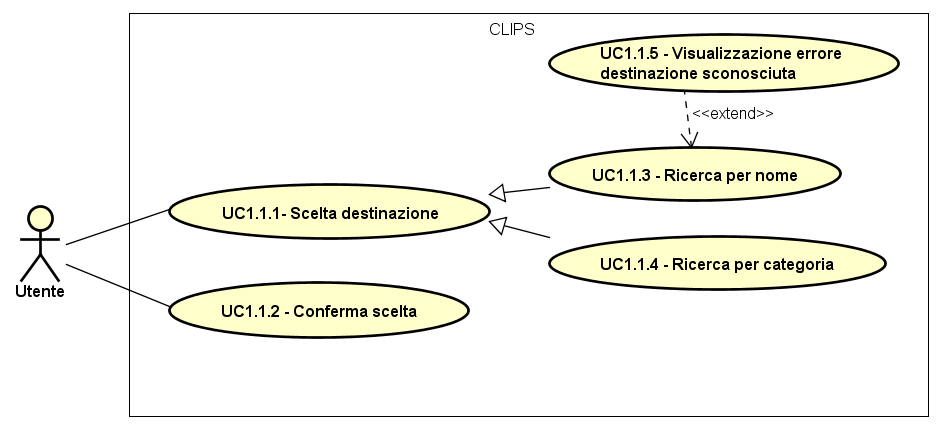
\includegraphics[scale=0.95, width=\textwidth]{img/UC1-1.png}
            \caption{Caso d'uso UC1.1: Inserimento destinazione}\label{fig:UC1.1} 
        \end{figure}
\begin{itemize}
\item \textbf{Attori}: utente;
\item \textbf{Descrizione}: l'utente deve poter scegliere ed inserire una destinazione da raggiungere, tra i POI previsti dall'edificio in cui si trova; 
      \item \textbf{Precondizione}: l'utente si trova nella sezione dedicata alla scelta della destinazione e il dispositivo rileva la presenza di un beacon;

        \item \textbf{Flusso principale degli eventi}:
          \begin{enumerate}
          \item L'utente sceglie una destinazione  (\hyperlink{UC1.1.1}{UC1.1.1});
          \item L'utente conferma la destinazione scelta  (\hyperlink{UC1.1.2}{UC1.1.2});

      \end{enumerate}
	 \item \textbf{Postcondizione}: la destinazione da raggiungere è stata impostata e confermata;
    \item \textbf{Scenari Alternativi}:
    	\begin{itemize}
    		\item Nel caso in cui l'utente ricerchi per nome un POI non appartenente all'edificio in cui si trova:
      		\begin{enumerate}
      			\item la destinazione inserita dall'utente non è riconosciuta dal sistema;
          		\item viene visualizzato un errore esplicativo (\hyperlink{UC1.1.5}{UC1.1.5});
          		\item viene data all'utente la possibilità di inserire una nuova destinazione.
      		\end{enumerate}
      	\end{itemize}
   
  \end{itemize}
\hypertarget{UC1.1.1}{}
\subsection{Caso d'uso UC1.1.1: Scelta destinazione}

\begin{itemize}
\item \textbf{Attori}: utente;

        \item \textbf{Generalizzazione di}:
          \begin{enumerate}
          \item l'utente deve poter inserire il nome di un POI che vuole raggiungere (\hyperlink{UC1.1.3}{UC1.1.3});
          \item l'utente deve poter cercare, tra le categorie proposte dal sistema, il POI che vuole raggiungere. Le categorie proposte sono relative all'edificio nel quale si trova l'utente (\hyperlink{UC1.1.4}{UC1.1.4});

      \end{enumerate}
\item \textbf{Descrizione}: l'utente deve poter scegliere una destinazione interna all'edificio, tra i POI conosciuti dal sistema; 
      \item \textbf{Precondizione}: l'utente si trova nella sezione dedicata all'inserimento della destinazione;

        \item \textbf{Flusso principale degli eventi}:
          \begin{enumerate}
          \item UC1.1.3: Ricerca per nome (\hyperlink{UC1.1.3}{UC1.1.3});
          \item UC1.1.4: Ricerca per categoria (\hyperlink{UC1.1.4}{UC1.1.4});

      \end{enumerate}
    \item \textbf{Postcondizione}: la destinazione è stata scelta.
  \end{itemize}
\hypertarget{UC1.1.2}{}
\subsection{Caso d'uso UC1.1.2: Conferma scelta}
\begin{itemize}
\item \textbf{Attori}: utente;
\item \textbf{Descrizione}: l'utente si trova nella sezione dedicata alla conferma della destinazione; 
      \item \textbf{Precondizione}: l'utente ha selezionato una destinazione, tra quelle previste dal sistema;

        \item \textbf{Flusso principale degli eventi}:
          \begin{enumerate}
          \item l'utente conferma di aver scelto un determinato POI come destinazione;

      \end{enumerate}
    \item \textbf{Postcondizione}: la destinazione scelta è stata confermata.
  \end{itemize}
\hypertarget{UC1.1.3}{}
\subsection{Caso d'uso UC1.1.3: Ricerca per nome}
\begin{itemize}
\item \textbf{Attori}: utente;
\item \textbf{Descrizione}: l'utente deve poter inserire il nome di una destinazione che vuole raggiungere; 
      \item \textbf{Precondizione}: l'utente si trova nella sezione dedicata alla ricerca per nome della destinazione;

        \item \textbf{Flusso principale degli eventi}:
          \begin{enumerate}
          \item l'utente inserisce il nome del POI che vuole raggiungere;

      \end{enumerate}

    \item \textbf{Postcondizione}: l'utente ha scelto la destinazione desiderata.
  \end{itemize}
\hypertarget{UC1.1.4}{}
\subsection{Caso d'uso UC1.1.4: Ricerca per categoria}
\begin{itemize}
\item \textbf{Attori}: utente;
\item \textbf{Descrizione}: l'utente deve poter cercare la destinazione che vuole raggiungere ricercandola tra le categorie di POI proposte dal sistema. Le categorie proposte dipendono dall'edificio nel quale si trova l'utente. Ad esempio, le categorie proposte da un edificio che ospita attività accademiche possono essere: aule, biblioteche, servizi igienici, laboratori ed uffici; 
      \item \textbf{Precondizione}: l'utente si trova nella sezione dedicata alla ricerca per categoria della destinazione;

        \item \textbf{Flusso principale degli eventi}:
          \begin{enumerate}
          \item l'utente sceglie una categoria tra quelle proposte;
          \item l'utente sceglie un POI tra quelli disponibili per la categoria scelta;

      \end{enumerate}
    \item \textbf{Postcondizione}: l'utente ha scelto la destinazione desiderata.
  \end{itemize}
\hypertarget{UC1.1.5}{}
\subsection{Caso d'uso UC1.1.5: Visualizzazione errore destinazione sconosciuta}
\begin{itemize}
\item \textbf{Attori}: utente;
\item \textbf{Descrizione}: l'utente ha indicato una destinazione sconosciuta al sistema; 
      \item \textbf{Precondizione}: L'utente ha digitato il nome di una destinazione sconosciuta al sistema;

        \item \textbf{Flusso principale degli eventi}:
          \begin{enumerate}
          \item viene visualizzato un errore esplicativo;

      \end{enumerate}
    \item \textbf{Postcondizione}: viene notificato all'utente che la destinazione indicata è sconosciuta al sistema.
  \end{itemize}
\hypertarget{UC1.2}{}
\subsection{Caso d'uso UC1.2: Avvio navigazione}
\begin{itemize}
\item \textbf{Attori}: utente;
\item \textbf{Descrizione}: l'utente deve poter avviare la navigazione in modo che il sistema calcoli il percorso e le relative indicazioni per guidare l'utente verso la destinazione scelta. Le indicazioni sono fornite in forma testuale; 
      \item \textbf{Precondizione}: l'utente ha inserito una destinazione valida e il dispositivo rileva la presenza di un beacon;

        \item \textbf{Flusso principale degli eventi}:
          \begin{enumerate}
          \item l'utente avvia la navigazione;
      \end{enumerate}
    \item \textbf{Inclusioni}:
      \begin{enumerate}
          \item Visualizzazione indicazioni (\hyperlink{UC1.5}{UC1.5});

      \end{enumerate}
    \item \textbf{Postcondizione}: il sistema ha fornito le indicazioni basilari  e necessarie all'utente per muoversi dalla sua posizione attuale alla destinazione scelta, rispettando le preferenze indicate dall'utente.
  \end{itemize}
\hypertarget{UC1.3}{}
\subsection{Caso d'uso UC1.3: Interruzione navigazione}
\begin{itemize}
\item \textbf{Attori}: utente;
\item \textbf{Descrizione}: l'utente deve poter interrompere la navigazione in corso; 
      \item \textbf{Precondizione}: l'utente ha avviato la navigazione;

        \item \textbf{Flusso principale degli eventi}:
          \begin{enumerate}
          \item l'utente interrompe la navigazione in corso;

      \end{enumerate}
    \item \textbf{Postcondizione}: la navigazione è stata interrotta e l'utente è stato riportato alla schermata principale dell'applicazione.
  \end{itemize}
\hypertarget{UC1.4}{}
\subsection{Caso d'uso UC1.4: Accesso a maggiori indicazioni}

        \begin{figure}[!h]
            \centering
            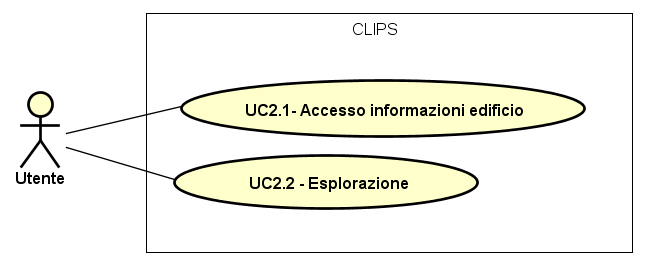
\includegraphics[scale=0.95, width=\textwidth]{img/UC1-4.png}
            \caption{Caso d'uso UC1.4: Accesso a maggiori indicazioni}\label{fig:UC1.4} 
        \end{figure}
\begin{itemize}
\item \textbf{Attori}: utente;
\item \textbf{Descrizione}: l'utente deve poter accedere ad indicazioni dettagliate che lo possano aiutare durante la navigazione; 
      \item \textbf{Precondizione}: l'utente ha avviato la navigazione e si trova nella sezione dedicata a fornire le informazioni più dettagliate;

        \item \textbf{Flusso principale degli eventi}:
          \begin{enumerate}
          \item L'utente può accede alle foto del prossimo POI (\hyperlink{UC1.4.1}{UC1.4.1});
          \item L'utente può accedere alle indicazioni testuali estese (\hyperlink{UC1.4.2}{UC1.4.2});
          \item L'utente può accedere alla lista delle indicazioni utili per raggiungere, dal POI in cui si trova, la destinazione scelta (\hyperlink{UC1.4.3}{UC1.4.3});

      \end{enumerate}
    \item \textbf{Postcondizione}: il sistema ha presentato all'utente informazioni dettagliate in supporto alla navigazione corrente.
  \end{itemize}
\hypertarget{UC1.4.1}{}
\subsection{Caso d'uso UC1.4.1: Accesso foto della prossima area}
\begin{itemize}
\item \textbf{Attori}: utente;
\item \textbf{Descrizione}: l'utente deve poter accedere alle foto che ritraggono il prossimo POI previsto dal percorso, in modo da poterlo individuare più facilmentente; 
      \item \textbf{Precondizione}: le foto relative al prossimo POI esistono e devono poter essere recuperate dall'applicazione;

        \item \textbf{Flusso principale degli eventi}:
          \begin{enumerate}
          \item l'utente accede alle foto che ritraggono il prossimo POI previsto dal percorso;

      \end{enumerate}
    \item \textbf{Postcondizione}: il sistema ha presentato all'utente le foto relative al prossimo POI.
  \end{itemize}
\hypertarget{UC1.4.2}{}
\subsection{Caso d'uso UC1.4.2: Accesso indicazione testuale estesa}
\begin{itemize}
\item \textbf{Attori}: utente;
\item \textbf{Descrizione}: l'utente deve poter accedere ad indicazioni più dettagliate che possano aiutarlo a raggiungere il prossimo POI previsto dal percorso; 
      \item \textbf{Precondizione}: le indicazioni dettagliate relative al prossimo POI esistono e devono poter essere recuperate dall'applicazione;

        \item \textbf{Flusso principale degli eventi}:
          \begin{enumerate}
          \item l'utente consulta le istruzioni dettagliate, utili a raggiungere il prossimo POI prevista dal percorso;

      \end{enumerate}
    \item \textbf{Postcondizione}: il sistema ha presentato all'utente indicazioni testuali dettagliate per raggiungere il prossimo POI.
  \end{itemize}
\hypertarget{UC1.4.3}{}
\subsection{Caso d'uso UC1.4.3: Accesso lista indicazioni}
\begin{itemize}
\item \textbf{Attori}: utente;
\item \textbf{Descrizione}: l'utente deve poter accedere alla lista completa delle indicazioni da seguire, a partire dal POI in cui si trova, per raggiungere la destinazione scelta. Tali indicazioni sono istruzioni utili all'utente per seguire il percorso, proposto dall'applicativo, dal POI in cui si trova alla destinazione scelta; 
      \item \textbf{Precondizione}: la lista che riporta tutte le indicazioni da seguire per raggiungere la destinazione, a partire dal POI in cui si trova l'utente, deve essere disponibile;

        \item \textbf{Flusso principale degli eventi}:
          \begin{enumerate}
          \item l'utente consulta la lista completa delle istruzioni per raggiungere la propria destinazione;

      \end{enumerate}
    \item \textbf{Postcondizione}: il sistema ha presentato all'utente la lista delle indicazioni richieste.
  \end{itemize}
\hypertarget{UC1.5}{}
\subsection{Caso d'uso UC1.5: Visualizzazione indicazioni}

\begin{itemize}
\item \textbf{Attori}: utente;
\item \textbf{Descrizione}: il sistema presenta all'utente le indicazioni utili alla navigazione. Tali indicazioni sono fondamentalmente istruzioni utili all'utente per seguire il percorso, proposto dall'applicativo, dal punto in cui si trova alla destinazione scelta; 
      \item \textbf{Precondizione}: l'utente ha avviato la navigazione;

        \item \textbf{Flusso principale degli eventi}:
          \begin{enumerate}
          \item l'utente consulta le indicazioni utili alla navigazione;

      \end{enumerate}

    \item \textbf{Postcondizione}: il sistema ha presentato all'utente le indicazioni per raggiungere la destinazione scelta.
  \end{itemize}
\hypertarget{UC1.6}{}
\subsection{Caso d'uso UC1.6: Visualizzazione errore percorso}
\begin{itemize}
\item \textbf{Attori}: utente;
\item \textbf{Descrizione}: viene visualizzato un errore che spiega all'utente che il percorso che sta prendendo non corrisponde al percorso calcolato; 
      \item \textbf{Precondizione}: i beacon rilevati dal sistema non corrispondono a quelli previsti dal percorso calcolato;

        \item \textbf{Flusso principale degli eventi}:
          \begin{enumerate}
          \item viene visualizzato un errore esplicativo;

      \end{enumerate}
    \item \textbf{Postcondizione}: il sistema ha presentato all'utente un errore relativo al percorso errato.
  \end{itemize}
\hypertarget{UC1.7}{}
\subsection{Caso d'uso UC1.7: Visualizzazione errore beacon}
\begin{itemize}
\item \textbf{Attori}: utente;
\item \textbf{Descrizione}: Viene visualizzato un errore che spiega all'utente che nell'area in cui si trova non è rilevato alcun beacon; 
      \item \textbf{Precondizione}: il dispositivo non è in grado di rilevare alcun beacon;

        \item \textbf{Flusso principale degli eventi}:
          \begin{enumerate}
          \item viene visualizzato un errore esplicativo;

      \end{enumerate}
    \item \textbf{Postcondizione}: il sistema ha presentato all'utente un errore relativo all'impossibilità di rilevare beacon.
  \end{itemize}
\hypertarget{UC2}{}
\subsection{Caso d'uso UC2: Accesso alle informazioni}

        \begin{figure}[!h]
            \centering
            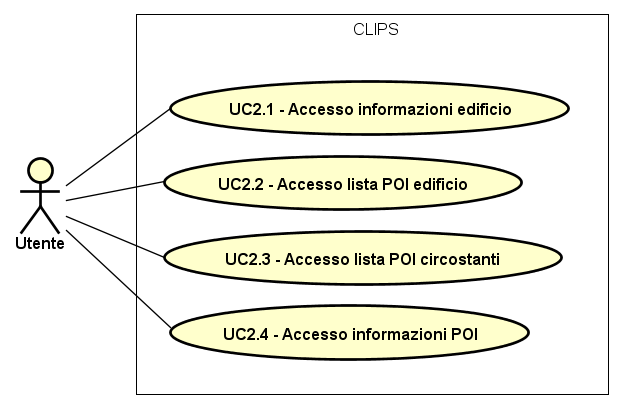
\includegraphics[scale=0.95, width=\textwidth]{img/UC2.png}
            \caption{Caso d'uso UC2: Accesso alle informazioni}\label{fig:UC2} 
        \end{figure}
\begin{itemize}
\item \textbf{Attori}: utente;
\item \textbf{Descrizione}: l'utente deve poter accedere alle informazioni riguardanti i POI vicini alla posizione in cui si trova. L'utente deve inoltre poter accedere alle informazioni relative all'edificio in cui si trova; 
      \item \textbf{Precondizione}: l'utente si trova nella sezione dedicata alle informazioni, ha attivato il Bluetooth, si trova all'interno di un edificio mappato e il dispositivo deve rilevare almeno un beacon;

        \item \textbf{Flusso principale degli eventi}:
          \begin{enumerate}
          \item L'utente può accedere alle informazioni dell'edificio (\hyperlink{UC2.1}{UC2.1});
          \item L'utente può accedere alla lista di tutti i POI presenti nell'edificio in cui si trova (\hyperlink{UC2.2}{UC2.2});
          \item l'utente deve poter accedere alla lista dei POI circostanti (\hyperlink{UC2.3}{UC2.3});
          \item l'utente deve poter accedere alle informazioni relative ad uno specifico POI (\hyperlink{UC2.4}{UC2.4});

      \end{enumerate}

    \item \textbf{Postcondizione}: il sistema ha presentato all'utente le informazioni richieste.
  \end{itemize}
\hypertarget{UC2.1}{}
\subsection{Caso d'uso UC2.1: Accesso alle informazioni dell'edificio}

        \begin{figure}[!h]
            \centering
            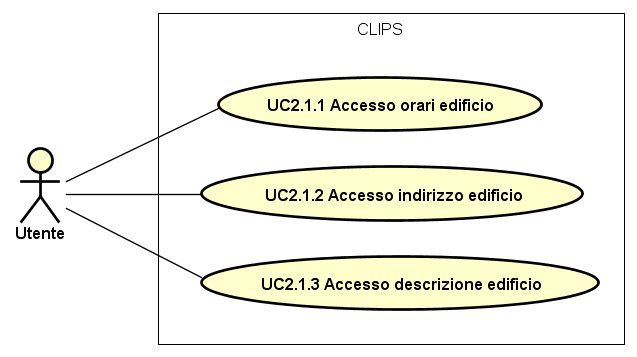
\includegraphics[scale=0.95, width=\textwidth]{img/UC2-1.png}
            \caption{Caso d'uso UC2.1: Accesso alle informazioni dell'edificio}\label{fig:UC2.1} 
        \end{figure}
\begin{itemize}
\item \textbf{Attori}: utente;
\item \textbf{Descrizione}: l'utente deve poter accedere alle informazioni riguardanti l'edificio in cui si trova; 
      \item \textbf{Precondizione}: l'utente si trova nella sezione relativa alle informazioni dell'edificio;

        \item \textbf{Flusso principale degli eventi}:
          \begin{enumerate}
          \item l'utente può accedere agli orari dell'edificio in cui si trova (\hyperlink{UC2.1.1}{UC2.1.1});
          \item l'utente può accedere all'indirizzo dell'edificio in cui si trova (\hyperlink{UC2.1.2}{UC2.1.2});
          \item l'utente può accedere al nome dell'edificio in cui si trova (\hyperlink{UC2.1.3}{UC2.1.3});
          \item l'utente può accedere alla descrizione dell'edificio in cui si trova (\hyperlink{UC2.1.4}{UC2.1.4});

      \end{enumerate}
    \item \textbf{Postcondizione}: il sistema ha presentato all'utente le informazioni sull'edificio.
  \end{itemize}
\hypertarget{UC2.1.1}{}
\subsection{Caso d'uso UC2.1.1: Accesso orari edificio}

\begin{itemize}
\item \textbf{Attori}: utente;
\item \textbf{Descrizione}: l'utente deve poter accedere agli orari di apertura dell'edificio in cui si trova; 
      \item \textbf{Precondizione}: l'utente si trova nella sezione adibita all'accesso delle informazioni dell'edificio;

        \item \textbf{Flusso principale degli eventi}:
          \begin{enumerate}
          \item l'utente accede agli orari di apertura dell'edificio in cui si trova;

      \end{enumerate}
    \item \textbf{Postcondizione}: il sistema ha presentato all'utente gli orari di apertura dell'edificio in cui si trova.
  \end{itemize}
\hypertarget{UC2.1.2}{}
\subsection{Caso d'uso UC2.1.2: Accesso indirizzo edificio}

\begin{itemize}
\item \textbf{Attori}: utente;
\item \textbf{Descrizione}: l’utente deve poter accedere all’indirizzo dell’edificio. L’indirizzo è così composto: via, numero civico, CAP(Codice di avviamento postale) e città.
      \item \textbf{Precondizione}: l'utente si trova nella sezione adibita all'accesso delle informazioni dell'edificio;

        \item \textbf{Flusso principale degli eventi}:
          \begin{enumerate}
          \item l'utente accede all'indirizzo dell'edificio in cui si trova;

      \end{enumerate}
    \item \textbf{Postcondizione}: il sistema ha presentato all'utente l'indirizzo dell'edificio in cui si trova.
  \end{itemize}
\hypertarget{UC2.1.3}{}
\subsection{Caso d'uso UC2.1.3: Accesso nome edificio}

\begin{itemize}
\item \textbf{Attori}: utente;
\item \textbf{Descrizione}: l'utente deve poter accedere al nome dell'edificio in cui si trova. Un edificio riceve un nome identificativo quando viene mappato da sensori beacon e inserito nel sistema CLIPS; 
      \item \textbf{Precondizione}: l'utente si trova nella sezione adibita all'accesso delle informazioni dell'edificio;

        \item \textbf{Flusso principale degli eventi}:
          \begin{enumerate}
          \item l'utente accede al nome dell'edificio in cui si trova;

      \end{enumerate}
    \item \textbf{Postcondizione}: il sistema ha presentato all'utente il nome dell'edificio in cui si trova.
  \end{itemize}
\hypertarget{UC2.1.4}{}
\subsection{Caso d'uso UC2.1.4: Accesso descrizione edificio}
\begin{itemize}
\item \textbf{Attori}: utente;
\item \textbf{Descrizione}: l'utente deve poter accedere alla descrizione dell'edificio in cui si trova. La descrizione comprende eventuali informazioni che il gestore dell'edificio vuole mettere a disposizione dell'utente; 
      \item \textbf{Precondizione}: l'utente si trova nella sezione adibita all'accesso delle informazioni dell'edificio;
    \item \textbf{Postcondizione}: il sistema ha presentato all'utente la descrizione dell'edificio in cui si trova.
  \end{itemize}
\hypertarget{UC2.2}{}
\subsection{Caso d'uso UC2.2: Accesso lista POI edificio}

\begin{itemize}
\item \textbf{Attori}: utente;
\item \textbf{Descrizione}: l'utente deve poter accedere alla lista di tutti i POI relativi all'edificio in cui si trova; 
      \item \textbf{Precondizione}: l'utente si trova nella sezione adibita all'accesso delle informazioni;

        \item \textbf{Flusso principale degli eventi}:
          \begin{enumerate}
          \item l'utente accede alla lista di tutti i POI relativi all'edificio in cui si trova;

      \end{enumerate}
    \item \textbf{Postcondizione}: il sistema ha presentato all'utente la lista di tutti i POI relativi all'edificio in cui si trova.
  \end{itemize}
\hypertarget{UC2.3}{}
\subsection{Caso d'uso UC2.3: Accesso lista POI circostanti}
\begin{itemize}
\item \textbf{Attori}: utente;
\item \textbf{Descrizione}: l'utente deve poter accedere alla lista dei POI circostanti, ovvero associati ai beacon rilevati; 
      \item \textbf{Precondizione}: l'utente si trova nella sezione adibita all'accesso delle informazioni;

        \item \textbf{Flusso principale degli eventi}:
          \begin{enumerate}
          \item l'utente accede alla lista dei POI circostanti;

      \end{enumerate}
    \item \textbf{Postcondizione}: il sistema ha presentato all'utente la lista dei POI circostanti.
  \end{itemize}
\hypertarget{UC2.4}{}
\subsection{Caso d'uso UC2.4: Accesso informazione POI}

        \begin{figure}[!h]
            \centering
            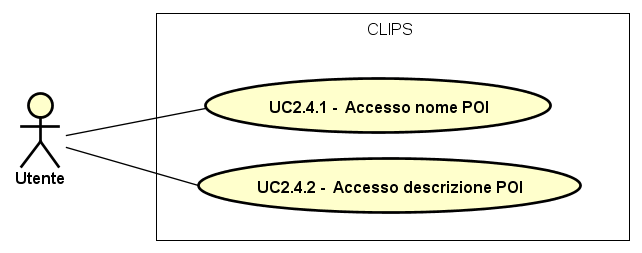
\includegraphics[scale=0.95, width=\textwidth]{img/UC2-4.png}
            \caption{Caso d'uso UC2.4: Accesso informazione POI}\label{fig:UC2.4} 
        \end{figure}
\begin{itemize}
\item \textbf{Attori}: utente;
\item \textbf{Descrizione}: l'utente deve poter accedere alle informazioni riguardanti uno specifico POI; 
      \item \textbf{Precondizione}: l'utente si trova nella sezione adibita all'accesso delle informazioni;

        \item \textbf{Flusso principale degli eventi}:
          \begin{enumerate}
          \item l'utente deve poter accedere al nome di uno specifico POI (\hyperlink{UC2.4.1}{UC2.4.1});
          \item l'utente può accedere alla descrizione di uno specifico POI (\hyperlink{UC2.4.2}{UC2.4.2});

      \end{enumerate}
    \item \textbf{Postcondizione}: il sistema ha presentato all'utente le informazioni riguardanti uno specifico POI.
  \end{itemize}
\hypertarget{UC2.4.1}{}
\subsection{Caso d'uso UC2.4.1: Accesso nome POI}

\begin{itemize}
\item \textbf{Attori}: utente;
\item \textbf{Descrizione}: l'utente deve poter accedere al nome di uno specifico POI. Un POI riceve un nome identificativo quando viene mappato con un sensore beacon e inserito nel sistema CLIPS.; 
      \item \textbf{Precondizione}: l'utente si trova nella sezione adibita all'accesso delle informazioni di uno specifico POI;

        \item \textbf{Flusso principale degli eventi}:
          \begin{enumerate}
          \item l'utente accede al nome di uno specifico POI;

      \end{enumerate}
    \item \textbf{Postcondizione}: il sistema ha presentato all'utente il nome di uno specifico POI.
  \end{itemize}
\hypertarget{UC2.4.2}{}
\subsection{Caso d'uso UC2.4.2: Accesso descrizione POI}
\begin{itemize}
\item \textbf{Attori}: utente;
\item \textbf{Descrizione}: l'utente deve poter accedere alla descrizione di uno specifico POI. La descrizione comprende eventuali informazioni che il gestore dell'edificio vuole mettere a disposizione dell'utente per quello specifico POI; 
      \item \textbf{Precondizione}: l'utente si trova nella sezione adibita all'accesso delle informazioni di uno specifico POI;

        \item \textbf{Flusso principale degli eventi}:
          \begin{enumerate}
          \item l'utente accede alla descrizione di uno specifico POI;

      \end{enumerate}
    \item \textbf{Postcondizione}: il sistema ha presentato all'utente la descrizione di uno specifico POI.
  \end{itemize}
\hypertarget{UC3}{}
\subsection{Caso d'uso UC3: Gestione dell'applicazione}

        \begin{figure}[!h]
            \centering
            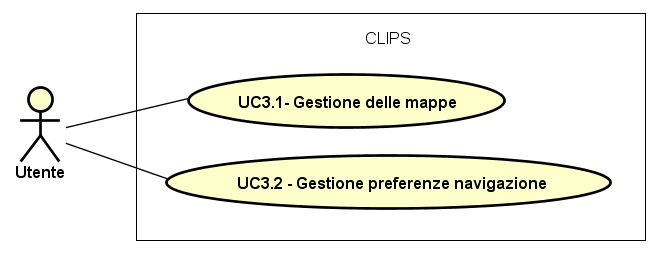
\includegraphics[scale=0.95, width=\textwidth]{img/UC3.png}
            \caption{Caso d'uso UC3: Gestione dell'applicazione}\label{fig:UC3} 
        \end{figure}
\begin{itemize}
\item \textbf{Attori}: utente;
\item \textbf{Descrizione}: l'utente deve poter gestire le mappe utilizzate dall'applicazione e le preferenze relative alle modalità di navigazione; 
      \item \textbf{Precondizione}: l'utente si trova nella sezione che ospita le opzioni per gestire l'applicazione;

        \item \textbf{Flusso principale degli eventi}:
          \begin{enumerate}
          \item L'utente può accedere alla gestione delle mappe (\hyperlink{UC3.1}{UC3.1});
          \item L'utente può accedere alla gestione delle preferenze di navigazione (\hyperlink{UC3.2}{UC3.2});

      \end{enumerate}
    \item \textbf{Postcondizione}: l'utente ha acceduto alla funzionalità richiesta.
  \end{itemize}
\hypertarget{UC3.1}{}
\subsection{Caso d'uso UC3.1: Gestione mappe}

        \begin{figure}[!h]
            \centering
            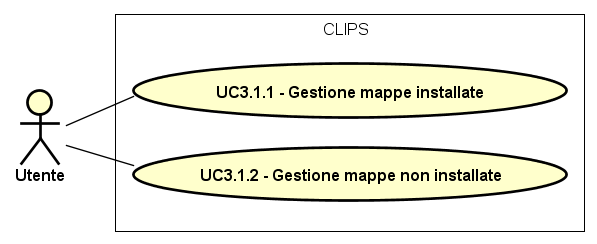
\includegraphics[scale=0.95, width=\textwidth]{img/UC3-1.png}
            \caption{Caso d'uso UC3.1: Gestione mappe}\label{fig:UC3.1} 
        \end{figure}
\begin{itemize}
\item \textbf{Attori}: utente;
\item \textbf{Descrizione}: l'utente deve poter gestire le mappe degli edifici, fondamentali al funzionamento dell'applicazione; 
      \item \textbf{Precondizione}: l'utente si trova nella sezione adibita alla gestione delle mappe;

        \item \textbf{Flusso principale degli eventi}:
          \begin{enumerate}
          \item L'utente può aggiornare una mappa scaricata in precedenza (\hyperlink{UC3.1.1}{UC3.1.1});
          \item L'utente può rimuovere una mappa scaricata in precedenza (\hyperlink{UC3.1.2}{UC3.1.2});
          \item L'utente può effettuare il download di una mappa sul proprio dispositivo (\hyperlink{UC3.1.3}{UC3.1.3});

      \end{enumerate}
    \item \textbf{Postcondizione}: il sistema ha erogato la funzionalità richiesta.
  \end{itemize}
\hypertarget{UC3.1.1}{}
\subsection{Caso d'uso UC3.1.1: Aggiornamento mappa scaricata}
\begin{itemize}
\item \textbf{Attori}: utente;

\item \textbf{Descrizione}: l'utente deve poter aggiornare la mappa di un edificio dgià presente sul proprio dispositivo; 
      \item \textbf{Precondizione}: il dispositivo dell'utente è provvisto di una connessione Internet attiva ed ha abbastanza spazio di archiviazione per la mappa aggiornata;
    \item \textbf{Postcondizione}: la mappa è stata aggiornata.
  \end{itemize}
\hypertarget{UC3.1.2}{}
\subsection{Caso d'uso UC3.1.2: Rimozione mappa scaricata}

\begin{itemize}
\item \textbf{Attori}: utente;
\item \textbf{Descrizione}: l'utente deve poter rimuovere dal dispositivo la mappa di un edificio scaricata in precedenza; 
      \item \textbf{Precondizione}: l'utente ha effettuato precedentemente il download della mappa;

        \item \textbf{Flusso principale degli eventi}:
          \begin{enumerate}
          \item l'utente rimuove la mappa;

      \end{enumerate}
    \item \textbf{Postcondizione}: la mappa è stata rimossa.
  \end{itemize}
\hypertarget{UC3.1.3}{}
\subsection{Caso d'uso UC3.1.3: Aggiunta nuova mappa}

        \begin{figure}[!h]
            \centering
            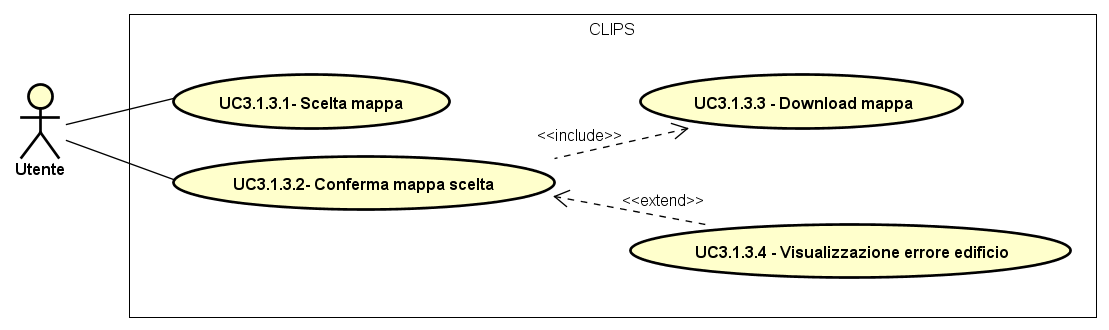
\includegraphics[scale=0.95, width=\textwidth]{img/UC3-1-3.png}
            \caption{Caso d'uso UC3.1.3: Aggiunta nuova mappa}\label{fig:UC3.1.3} 
        \end{figure}
\begin{itemize}
\item \textbf{Attori}: utente;
\item \textbf{Descrizione}: l'utente deve poter effettuare il download della mappa relativa ad uno specifico edificio; 
      \item \textbf{Precondizione}: il dispositivo dell'utente è provvisto di una connessione Internet attiva ed ha abbastanza spazio di archiviazione per la nuova mappa;

        \item \textbf{Flusso principale degli eventi}:
          \begin{enumerate}
          \item L'utente sceglie una mappa tra quelle disponibili (\hyperlink{UC3.1.3.1}{UC3.1.3.1});
          \item L'utente conferma la mappa scelta  (\hyperlink{UC3.1.3.2}{UC3.1.3.2});

      \end{enumerate}
    \item \textbf{Postcondizione}: la mappa è stata scaricata sul dispositivo dell'utente ed il sistema può utilizzarla;
    \item \textbf{Scenari Alternativi}:
    	\begin{itemize}
			\item Nel caso in cui l'utente richieda la mappa di un edificio sconosciuto al sistema:
			\begin{enumerate}
				\item Viene visualizzato un errore riguardante l'edificio scelto (\hyperlink{UC3.1.3.4}{UC3.1.3.4});
				\item viene data la possibilità all'utente di scegliere un'altra mappa di cui effettuare il download.
			\end{enumerate}
      	\end{itemize}
  \end{itemize}
\hypertarget{UC3.1.3.1}{}
\subsection{Caso d'uso UC3.1.3.1: Scelta mappa}
\begin{itemize}
\item \textbf{Attori}: utente;
\item \textbf{Descrizione}: l'utente deve poter scegliere la mappa relativa ad un certo edificio; 
      \item \textbf{Precondizione}: l'utente è nella sezione dedicata alla scelta delle mappe;

        \item \textbf{Flusso principale degli eventi}:
          \begin{enumerate}
          \item l'utente sceglie l'edificio del quale vuole scaricare la mappa;

      \end{enumerate}
    \item \textbf{Postcondizione}: l'utente ha scelto la mappa dell'edificio desiderato.
  \end{itemize}
\hypertarget{UC3.1.3.2}{}
\subsection{Caso d'uso UC3.1.3.2: Conferma mappa scelta}
\begin{itemize}
\item \textbf{Attori}: utente;
\item \textbf{Descrizione}: l'utente deve poter confermare la mappa scelta per poterne effettuare il download; 
      \item \textbf{Precondizione}: l'utente è nella sezione dedicata alla scelta delle mappe;

        \item \textbf{Flusso principale degli eventi}:
          \begin{enumerate}
          \item l'utente conferma la scelta della mappa da scaricare;        

      \end{enumerate}
    \item \textbf{Inclusioni}:
      \begin{enumerate}
          \item Download mappa (\hyperlink{UC3.1.3.3}{UC3.1.3.3});

      \end{enumerate}

    \item \textbf{Postcondizione}: l'utente ha scelto la mappa dell'edificio desiderato.
  \end{itemize}
\hypertarget{UC3.1.3.3}{}
\subsection{Caso d'uso UC3.1.3.3: Download mappa}
\begin{itemize}
\item \textbf{Attori}: utente;
\item \textbf{Descrizione}: L'utente deve poter effettuare il download della mappa scelta; 
      \item \textbf{Precondizione}: l'utente ha confermato la mappa da scaricare ed ha abbastanza spazio di archiviazione per la nuova mappa;

        \item \textbf{Flusso principale degli eventi}:
          \begin{enumerate}
          \item il sistema procede al download della mappa;

      \end{enumerate}
    \item \textbf{Postcondizione}: la mappa è stata scaricata ed è presente nel dispositivo dell'utente.
  \end{itemize}
\hypertarget{UC3.1.3.4}{}
\subsection{Caso d'uso UC3.1.3.4: Visualizzazione errore edificio}
\begin{itemize}
\item \textbf{Attori}: utente;
\item \textbf{Descrizione}: all'utente viene presentato un errore che spiega che la mappa per l'edificio inserito non è presente oppure che il nome dell'edificio inserito non è corretto, dando la possibilità all'utente di inserire il nome di un altro edificio; 
      \item \textbf{Precondizione}: l'utente ha richiesto la mappa di un edificio non riconosciuto dal sistema;

        \item \textbf{Flusso principale degli eventi}:
          \begin{enumerate}
          \item viene visualizzato un errore esplicativo;

      \end{enumerate}
    \item \textbf{Postcondizione}: il sistema visualizza un messaggio di errore riguardante l'impossibilità di trovare la mappa relativa all'edificio scelto.
  \end{itemize}
\hypertarget{UC3.2}{}
\subsection{Caso d'uso UC3.2: Gestione preferenze navigazione}

        \begin{figure}[!h]
            \centering
            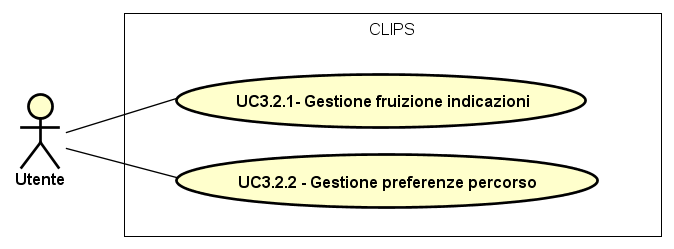
\includegraphics[scale=0.95, width=\textwidth]{img/UC3-2.png}
            \caption{Caso d'uso UC3.2: Gestione preferenze navigazione}\label{fig:UC3.2} 
        \end{figure}
\begin{itemize}
\item \textbf{Attori}: utente;
\item \textbf{Descrizione}: l'utente deve poter gestire le preferenze rispetto a come l'applicazione fornisce indicazioni durante la navigazione e rispetto alle caratteristiche desiderabili che un percorso proposto dovrebbe avere; 
      \item \textbf{Precondizione}: l'utente si trova nella sezione dedicata alla gestione delle preferenze di navigazione;

        \item \textbf{Flusso principale degli eventi}:
          \begin{enumerate}
          \item L'utente può gestire il modo in cui preferisce che le indicazioni gli siano presentate durante la navigazione (\hyperlink{UC3.2.1}{UC3.2.1});
          \item L'utente può gestire le qualità desiderabili che un percorso proposto dovrebbe avere (\hyperlink{UC3.2.2}{UC3.2.2});

      \end{enumerate}
    \item \textbf{Postcondizione}: le preferenze indicate dall'utente riguardo la navigazione sono note al sistema e verranno applicate a partire dalla prossima volta che l'utente avvierà la navigazione.
  \end{itemize}
\hypertarget{UC3.2.1}{}
\subsection{Caso d'uso UC3.2.1: Gestione fruizione indicazioni}

        \begin{figure}[!h]
            \centering
            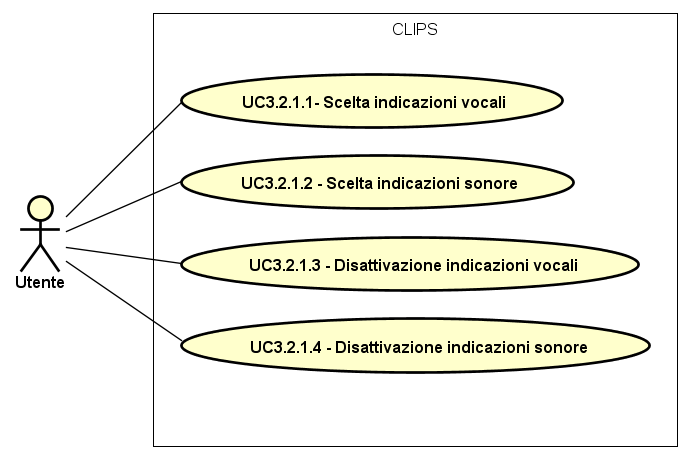
\includegraphics[scale=0.95, width=\textwidth]{img/UC3-2-1.png}
            \caption{Caso d'uso UC3.2.1: Gestione fruizione indicazioni}\label{fig:UC3.2.1} 
        \end{figure}
\begin{itemize}
\item \textbf{Attori}: utente;
\item \textbf{Descrizione}: l'utente deve poter scegliere la modalità tramite la quale preferisce ricevere le indicazioni quando si trova in navigazione; 
      \item \textbf{Precondizione}: l'utente si trova nella sezione dedicata alla gestione della fruizione delle indicazioni;

        \item \textbf{Flusso principale degli eventi}:
          \begin{enumerate}
          \item L'utente può scegliere di attivare indicazioni vocali (\hyperlink{UC3.2.1.1}{UC3.2.1.1});
          \item L'utente può scegliere di attivare indicazioni sonore (\hyperlink{UC3.2.1.2}{UC3.2.1.2});
          \item L'utente può scegliere di disattivare le indicazioni vocali (\hyperlink{UC3.2.1.3}{UC3.2.1.3});
          \item L'utente può scegliere di disattivare le indicazioni sonore (\hyperlink{UC3.2.1.4}{UC3.2.1.4});
      \end{enumerate}
    \item \textbf{Postcondizione}: le preferenze dell'utente rispetto alla fruizione delle indicazioni sono note al sistema e verranno applicate a partire dalla prossima volta che l'utente avvierà la navigazione.
  \end{itemize}
\hypertarget{UC3.2.1.1}{}
\subsection{Caso d'uso UC3.2.1.1: Attivazione indicazioni vocali}
\begin{itemize}
\item \textbf{Attori}: utente;
\item \textbf{Descrizione}: l'utente deve poter scegliere di attivare le indicazioni vocali che lo guidino alla destinazione scelta; 
      \item \textbf{Precondizione}: le indicazioni vocali sono disponibili e non sono precedentemente state attivate;

        \item \textbf{Flusso principale degli eventi}:
          \begin{enumerate}
          \item l'utente attiva le indicazioni vocali;

      \end{enumerate}
    \item \textbf{Postcondizione}: il sistema fornirà indicazioni vocali partire dalla prossima volta in cui l'utente avvierà la navigazione.
  \end{itemize}
\hypertarget{UC3.2.1.2}{}
\subsection{Caso d'uso UC3.2.1.2: Attivazione indicazioni sonore}
\begin{itemize}
\item \textbf{Attori}: utente;
\item \textbf{Descrizione}: l'utente deve poter scegliere di attivare le indicazioni sonore che lo guidino alla destinazione scelta. Questo indicazioni consisteno nell'emissione di un suono monotono continuo quando l'utente segue il percorso previsto. Quando invece un utente si allontanerà dal percorso previsto, la cui frequenza del suono varierà. Questo tipo di indicazioni è pensato per agevolare la navigazione di utenti che presentano disabilità visive; 
      \item \textbf{Precondizione}: le indicazioni sonore sono disponibili e non sono state precedentemente attivate;

        \item \textbf{Flusso principale degli eventi}:
          \begin{enumerate}
          \item l'utente attiva le indicazioni sonore;
      \end{enumerate}
    \item \textbf{Postcondizione}: il sistema fornirà indicazioni sonore a partire dalla prossima volta in cui l'utente avvierà la navigazione.
  \end{itemize}
\hypertarget{UC3.2.1.3}{}
\subsection{Caso d'uso UC3.2.1.3: Disattivazione indicazioni vocali}
\begin{itemize}
\item \textbf{Attori}: utente;
\item \textbf{Descrizione}: l'utente deve poter scegliere di disattivare le indicazioni vocali; 
      \item \textbf{Precondizione}: le indicazioni vocali sono state precedentemente attivate;
      \item \textbf{Flusso principale degli eventi}:
          \begin{enumerate}
          \item l'utente disattiva le indicazioni vocali;
      \end{enumerate}
    \item \textbf{Postcondizione}: il sistema non fornirà le indicazioni vocali a partire dalla prossima volta che l'utente avvierà la navigazione.
  \end{itemize}
\hypertarget{UC3.2.1.4}{}
\subsection{Caso d'uso UC3.2.1.4: Disattivazione indicazioni sonore}
\begin{itemize}
\item \textbf{Attori}: utente;
\item \textbf{Descrizione}: l'utente deve poter scegliere di disattivare le indicazioni sonore che lo guidino alla destinazione scelta; 
      \item \textbf{Precondizione}: le indicazioni sonore sono state precedentemente attivate;
      \item \textbf{Flusso principale degli eventi}:
          \begin{enumerate}
          \item l'utente disattiva le indicazioni sonore;
      \end{enumerate}
    \item \textbf{Postcondizione}: il sistema non fornirà le indicazioni sonore a partire dalla prossima volta in cui l'utente avvierà la navigazione.
  \end{itemize}
\hypertarget{UC3.2.2}{}
\subsection{Caso d'uso UC3.2.2: Gestione preferenze percorso}

        \begin{figure}[!h]
            \centering
            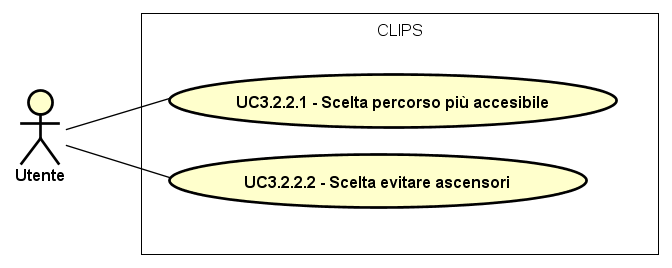
\includegraphics[scale=0.95, width=\textwidth]{img/UC3-2-2.png}
            \caption{Caso d'uso UC3.2.2: Gestione preferenze percorso}\label{fig:UC3.2.2} 
        \end{figure}
\begin{itemize}
\item \textbf{Attori}: utente;
\item \textbf{Descrizione}: l'utente deve poter scegliere le caratteristiche desiderabili che un percorso proposto dovrebbe avere. Queste caratteristiche permettono al sistema di calcolare il percorso più adatto alle necessità dell'utente; 
      \item \textbf{Precondizione}: l'utente si trova nella sezione dedicata alla gestione delle preferenze di percorso;

        \item \textbf{Flusso principale degli eventi}:
          \begin{enumerate}
          \item L'utente può indicare che preferisce il percorso più accessibile (\hyperlink{UC3.2.2.1}{UC3.2.2.1});
          \item L'utente può indicare che preferisce percorsi che non prevedano spazi chiusi e ristretti  (\hyperlink{UC3.2.2.2}{UC3.2.2.2});

      \end{enumerate}
    \item \textbf{Postcondizione}: le preferenze dell'utente rispetto al percorso sono note al sistema e verranno applicate a partire dalla prossima volta che l'utente avvierà la navigazione.
  \end{itemize}
\hypertarget{UC3.2.2.1}{}
\subsection{Caso d'uso UC3.2.2.1: Scelta percorso più accessibile}
\begin{itemize}
\item \textbf{Attori}: utente;
\item \textbf{Descrizione}: l'utente deve poter scegliere di ricevere indicazioni per il percorso più accessibile. Il percorso più accessibile è quello che presenta meno barriere architettoniche. Questo tipo di indicazioni è pensato per agevolare la navigazione di utenti che presentano disabilità motorie; 
      \item \textbf{Precondizione}: l'utente si trova nella sezione dedicata alla gestione delle preferenze di percorso;
      \item \textbf{Flusso principale degli eventi}:
          \begin{enumerate}
          \item l'utente sceglie il percorso più accessibile;
      \end{enumerate}
    \item \textbf{Postcondizione}: il sistema calcolerà il percorso più accessibile a partire dalla prossima volta che l'utente avvierà la navigazione.
  \end{itemize}
\hypertarget{UC3.2.2.2}{}
\subsection{Caso d'uso UC3.2.2.2: Scelta evitare ascensori}
\begin{itemize}
\item \textbf{Attori}: utente;
\item \textbf{Descrizione}: l'utente deve poter scegliere di ricevere indicazioni per il percorso che presenta il minor numero di ascensori. Questo tipo di indicazioni è pensato per agevolare la navigazione di utenti claustrofobici; 
      \item \textbf{Precondizione}: l'utente si trova nella sezione dedicata alla gestione delle preferenze di percorso;
      \item \textbf{Flusso principale degli eventi}:
          \begin{enumerate}
          \item l'utente sceglie il percorso che prevede il minor numero di ascensori;
      \end{enumerate}
    \item \textbf{Postcondizione}: il sistema calcolerà il percorso col minor numero di ascensori a partire dalla prossima volta che l'utente avvierà la navigazione.
  \end{itemize}
\hypertarget{UC4}{}
\subsection{Caso d'uso UC4: Attivazione funzionalità sviluppatore}

        \begin{figure}[!h]
            \centering
            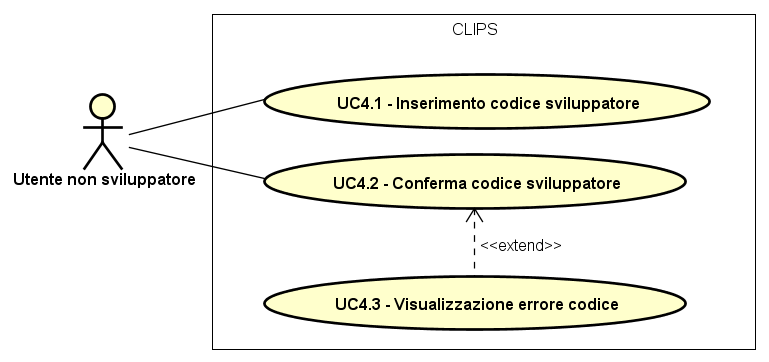
\includegraphics[scale=0.95, width=\textwidth]{img/UC4.png}
            \caption{Caso d'uso UC4: Attivazione funzionalità sviluppatore}\label{fig:UC4} 
        \end{figure}
\begin{itemize}
\item \textbf{Attori}: utente non sviluppatore;
\item \textbf{Descrizione}: un utente, se è in possesso di un codice sviluppatore valido, deve poter attivare le funzionalità avanzate dedicate agli sviluppatori offerte dall'applicazione; 
      \item \textbf{Precondizione}: l'utente si trova nella sezione dedicata all'attivazione delle funzionalità sviluppatore e l'utente non è già sviluppatore;

        \item \textbf{Flusso principale degli eventi}:
          \begin{enumerate}
          \item L'utente inserisce il codice sviluppatore (\hyperlink{UC4.1}{UC4.1});
          \item L'utente conferma il codice inserito (\hyperlink{UC4.2}{UC4.2});

      \end{enumerate}
   \item \textbf{Postcondizione}: il sistema rende disponibili le funzionalità avanzate, riservate agli sviluppatori;
    \item \textbf{Scenari Alternativi}:
    	\begin{itemize}
    		\item Nel caso in cui l'utente inserisca un codice sviluppatore non valido:
    		\begin{enumerate}
    			\item Viene visualizzato un errore riguardante il codice inserito (\hyperlink{UC4.3}{UC4.3});
    			\item viene data la possibilità di inserire nuovamente un codice.
    			
    		\end{enumerate}
    	\end{itemize}

 
  \end{itemize}
\hypertarget{UC4.1}{}
\subsection{Caso d'uso UC4.1: Inserimento codice sviluppatore}

\begin{itemize}
\item \textbf{Attori}: utente non sviluppatore;
\item \textbf{Descrizione}: l'utente deve poter inserire un codice così da accedere alle funzionalità sviluppatore; 
      \item \textbf{Precondizione}: l'utente non ha mai inserito un codice valido prima;

        \item \textbf{Flusso principale degli eventi}:
          \begin{enumerate}
          \item l'utente inserisce un codice di attivazione;

      \end{enumerate}
    \item \textbf{Postcondizione}: il codice sviluppatore è stato inserito.
  \end{itemize}
\hypertarget{UC4.2}{}
\subsection{Caso d'uso UC4.2: Conferma codice}

\begin{itemize}
\item \textbf{Attori}: utente non sviluppatore;
\item \textbf{Descrizione}: l'utente deve poter confermare il codice sviluppatore inserito; 
      \item \textbf{Precondizione}: l'utente ha inserito un codice nell'apposita sezione;

        \item \textbf{Flusso principale degli eventi}:
          \begin{enumerate}
          \item l'utente conferma il codice di attivazione inserito;

      \end{enumerate}
    
    \item \textbf{Postcondizione}: il sistema permette l'accesso alle funzionalità sviluppatore.
  \end{itemize}
\hypertarget{UC4.3}{}
\subsection{Caso d'uso UC4.3: Visualizzazione errore codice}
\begin{itemize}
\item \textbf{Attori}: utente non sviluppatore;
\item \textbf{Descrizione}: viene visualizzato un errore che spiega all'utente che il codice inserito non è riconosciuto come un codice valido per attivare le funzioni di sviluppatore; 
      \item \textbf{Precondizione}: l'utente ha inserito un codice sviluppatore non valido;

        \item \textbf{Flusso principale degli eventi}:
          \begin{enumerate}
          \item viene visualizzato un errore esplicativo;
      \end{enumerate}
    \item \textbf{Postcondizione}: il sistema non permette l'accesso alle funzionalità sviluppatore.
  \end{itemize}
\hypertarget{UC5}{}
\subsection{Caso d'uso UC5: Accesso alla guida}
\begin{itemize}
\item \textbf{Attori}: utente;
\item \textbf{Descrizione}: l'utente deve poter accedere ad una guida che illustri l'utilizzo del prototipo; 
      \item \textbf{Precondizione}: il sistema mette a disposizione una sezione che ospita la guida;

        \item \textbf{Flusso principale degli eventi}:
          \begin{enumerate}
          \item l'utente accede alla guida;

      \end{enumerate}
    \item \textbf{Postcondizione}: il sistema ha presentato la guida all'utente.
  \end{itemize}
\hypertarget{UC6}{}
\subsection{Caso d'uso UC6: Accesso funzionalità sviluppatore}

        \begin{figure}[!h]
            \centering
            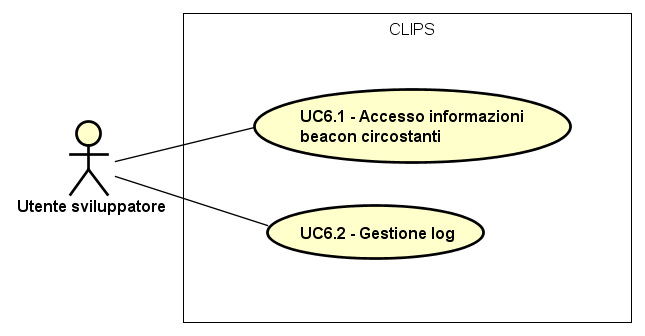
\includegraphics[scale=0.95, width=\textwidth]{img/UC6.png}
            \caption{Caso d'uso UC6: Accesso funzionalità sviluppatore}\label{fig:UC6} 
        \end{figure}
\begin{itemize}
\item \textbf{Attori}: utente sviluppatore;
\item \textbf{Descrizione}: lo sviluppatore deve poter accedere alle funzionalità avanzate messe a disposizione dall'applicazione. Tali funzionalità sono rivolte a testare e migliorare l'applicazione ed il sistema dei beacon con cui interagisce; 
      \item \textbf{Precondizione}: lo sviluppatore si trova nella sezione dedicata alle funzionalità avanzate dell'applicazione;

        \item \textbf{Flusso principale degli eventi}:
          \begin{enumerate}
          \item Lo sviluppatore può accedere alle informazioni relative ai beacon circostanti (\hyperlink{UC6.1}{UC6.1});
          \item Lo sviluppatore può gestire i log (\hyperlink{UC6.2}{UC6.2});

      \end{enumerate}
    \item \textbf{Postcondizione}: lo sviluppatore ha usufruito delle funzionalità avanzate.
  \end{itemize}
\hypertarget{UC6.1}{}
\subsection{Caso d'uso UC6.1: Accesso informazioni beacon circostanti}
\begin{figure}[!h]
            \centering
            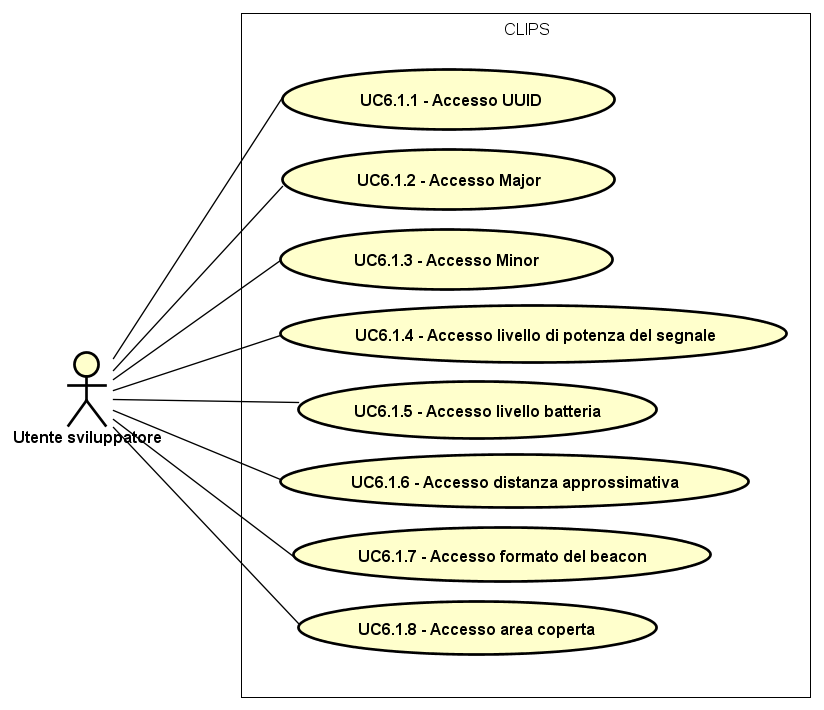
\includegraphics[scale=0.95, width=\textwidth]{img/UC6-1.png}
            \caption{Caso d'uso UC6: Accesso funzionalità sviluppatore}\label{fig:UC6} 
        \end{figure}
\begin{itemize}
\item \textbf{Attori}: utente sviluppatore;
\item \textbf{Descrizione}: lo sviluppatore deve poter accedere alle informazioni relative ai beacon presenti nelle vicinanze. Tali informazioni riguardano: UUID, Major, Minor, livello di potenza del segnale, livello batteria, distanza approssimativa, formato del beacon, area coperta dal beacon; 
      \item \textbf{Precondizione}: lo sviluppatore si trova nella sezione dedicata alle informazioni sui beacon circostanti, ha il Bluetooth attivato ed il dispositivo rileva almeno un beacon;
    \item \textbf{Postcondizione}: lo sviluppatore ha avuto accesso alle informazioni relative ai beacon circostanti.
  \end{itemize}
\hypertarget{UC6.1.1}{}
\subsection{Caso d'uso UC6.1.1: Accesso UUID}
\begin{itemize}
\item \textbf{Attori}: utente sviluppatore;
\item \textbf{Descrizione}: Lo sviluppatore deve poter accedere al UUID di un beacon nelle vicinanze; 
      \item \textbf{Precondizione}: Lo sviluppatore si trova nella sezione dedicata all'accesso alle informazioni dei beacon circostanti;

        \item \textbf{Flusso principale degli eventi}:
          \begin{enumerate}
          \item lo sviluppatore accede all'UUID di un beacon circostante;

      \end{enumerate}
    \item \textbf{Postcondizione}: Lo sviluppatore ha avuto accesso all'UUID.
  \end{itemize}
\hypertarget{UC6.1.2}{}
\subsection{Caso d'uso UC6.1.2: Accesso Major}

\begin{itemize}
\item \textbf{Attori}: utente sviluppatore;
\item \textbf{Descrizione}: Lo sviluppatore deve poter accedere al Major di un beacon nelle vicinanze; 
      \item \textbf{Precondizione}: Lo sviluppatore si trova nella sezione dedicata all'accesso alle informazioni dei beacon circostanti;

        \item \textbf{Flusso principale degli eventi}:
          \begin{enumerate}
          \item Lo sviluppatore accede al Major di un beacon nelle vicinanze;

      \end{enumerate}
    \item \textbf{Postcondizione}: Lo sviluppatore ha avuto accesso al Major.
  \end{itemize}
\hypertarget{UC6.1.3}{}
\subsection{Caso d'uso UC6.1.3: Accesso Minor}


\begin{itemize}
\item \textbf{Attori}: utente sviluppatore;
\item \textbf{Descrizione}: Lo sviluppatore deve poter accedere al Minor di un beacon nelle vicinanze; 
      \item \textbf{Precondizione}: Lo sviluppatore si trova nella sezione dedicata all'accesso alle informazioni dei beacon circostanti;

        \item \textbf{Flusso principale degli eventi}:
          \begin{enumerate}
          \item Lo sviluppatore accede al Minor di un beacon nelle vicinanze;

      \end{enumerate}
    \item \textbf{Postcondizione}: Lo sviluppatore ha avuto accesso al Minor.
  \end{itemize}
\hypertarget{UC6.1.4}{}
\subsection{Caso d'uso UC6.1.4: Accesso livello di potenza del segnale}
\begin{itemize}
\item \textbf{Attori}: utente sviluppatore;
\item \textbf{Descrizione}: Lo sviluppatore deve poter accedere al livello di potenza del segnale di un beacon nelle vicinanze; 
      \item \textbf{Precondizione}: Lo sviluppatore si trova nella sezione dedicata all'accesso alle informazioni dei beacon circostanti;

        \item \textbf{Flusso principale degli eventi}:
          \begin{enumerate}
          \item Lo sviluppatore accede al livello di potenza del segnale di un beacon nelle vicinanze;

      \end{enumerate}
    \item \textbf{Postcondizione}: Lo sviluppatore ha avuto accesso al livello di potenza.
  \end{itemize}
\hypertarget{UC6.1.5}{}
\subsection{Caso d'uso UC6.1.5: Accesso livello batteria}

\begin{itemize}
\item \textbf{Attori}: utente sviluppatore;
\item \textbf{Descrizione}: Lo sviluppatore deve poter accedere al livello della batteria di un beacon nelle vicinanze; 
      \item \textbf{Precondizione}: Lo sviluppatore si trova nella sezione dedicata all'accesso alle informazioni dei beacon circostanti;

        \item \textbf{Flusso principale degli eventi}:
          \begin{enumerate}
          \item Lo sviluppatore accede al livello della batteria di un beacon nelle vicinanze;

      \end{enumerate}
    \item \textbf{Postcondizione}: Lo sviluppatore ha avuto accesso al livello della batteria.
  \end{itemize}
\hypertarget{UC6.1.6}{}
\subsection{Caso d'uso UC6.1.6: Accesso distanza approssimativa}
\begin{itemize}
\item \textbf{Attori}: utente sviluppatore;
\item \textbf{Descrizione}: Lo sviluppatore deve poter accedere al valore della distanza approssimativa che esiste tra esso ed un beacon nelle vicinanze; 
      \item \textbf{Precondizione}: Lo sviluppatore si trova nella sezione dedicata all'accesso alle informazioni dei beacon circostanti;

        \item \textbf{Flusso principale degli eventi}:
          \begin{enumerate}
          \item Lo sviluppatore accede al valore della distanza approssimativa;

      \end{enumerate}
    \item \textbf{Postcondizione}: Lo sviluppatore ha avuto accesso al valore della distanza approssimativa.
  \end{itemize}
\hypertarget{UC6.1.7}{}
\subsection{Caso d'uso UC6.1.7: Accesso formato del beacon}

\begin{itemize}
\item \textbf{Attori}: utente sviluppatore;
\item \textbf{Descrizione}: Lo sviluppatore deve poter accedere al formato di un beacon nelle vicinanze; 
      \item \textbf{Precondizione}: Lo sviluppatore si trova nella sezione dedicata all'accesso alle informazioni dei beacon circostanti;

        \item \textbf{Flusso principale degli eventi}:
          \begin{enumerate}
          \item Lo sviluppatore accede al formato di un beacon nelle vicinanze;

      \end{enumerate}
    \item \textbf{Postcondizione}: Lo sviluppatore ha avuto accesso al formato di un beacon.
  \end{itemize}
\hypertarget{UC6.1.8}{}
\subsection{Caso d'uso UC6.1.8: Accesso area coperta da beacon}
\begin{itemize}
\item \textbf{Attori}: utente sviluppatore;
\item \textbf{Descrizione}: Lo sviluppatore deve potere accedere all’area di copertura di un beacon nelle vicinanze; 
      \item \textbf{Precondizione}: Lo sviluppatore si trova nella sezione dedicata all'accesso alle informazioni dei beacon circostanti;

        \item \textbf{Flusso principale degli eventi}:
          \begin{enumerate}
          \item Lo sviluppatore accede all’area di copertura di un beacon nelle vicinanze;

      \end{enumerate}
    \item \textbf{Postcondizione}: Lo sviluppatore ha avuto accesso all’area di copertura di un beacon.
  \end{itemize}
\hypertarget{UC6.2}{}
\subsection{Caso d'uso UC6.2: Gestione log}

        \begin{figure}[!h]
            \centering
            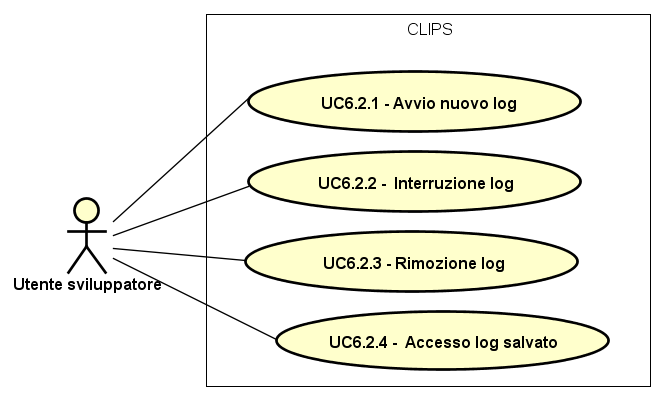
\includegraphics[scale=0.95, width=\textwidth]{img/UC6-2.png}
            \caption{Caso d'uso UC6.2: Gestione log}\label{fig:UC6.2} 
        \end{figure}
\begin{itemize}
\item \textbf{Attori}: utente sviluppatore;
\item \textbf{Descrizione}: lo sviluppatore deve poter accedere alla gestione del log. Il log contiene tutte le informazioni indicate in UC6.1 e relative ai beacon rilevati durante la registrazione del log. Lo sviluppatore può decidere quando avviare e interrompere la registrazione del log; 
      \item \textbf{Precondizione}: lo sviluppatore si trova nella sezione dedicata alla gestione del log;

        \item \textbf{Flusso principale degli eventi}:
          \begin{enumerate}
          \item Lo sviluppatore può avviare un nuovo log (\hyperlink{UC6.2.1}{UC6.2.1});
          \item Lo sviluppatore può interrompere un log in corso (\hyperlink{UC6.2.2}{UC6.2.2});
          \item Lo sviluppatore può rimuovere un log salvato (\hyperlink{UC6.2.3}{UC6.2.3});
          \item Lo sviluppatore può accedere ad un log salvato (\hyperlink{UC6.2.4}{UC6.2.4});

      \end{enumerate}
    \item \textbf{Postcondizione}: lo sviluppatore ha usufruito della gestione del log.
  \end{itemize}
\hypertarget{UC6.2.1}{}
\subsection{Caso d'uso UC6.2.1: Avvio nuovo log}

\begin{itemize}
\item \textbf{Attori}: utente sviluppatore;
\item \textbf{Descrizione}: lo sviluppatore deve poter avviare un nuovo log; 
      \item \textbf{Precondizione}: lo sviluppatore si trova nella sezione dedicata alla gestione dei log;

        \item \textbf{Flusso principale degli eventi}:
          \begin{enumerate}
          \item lo sviluppatore avvia un nuovo log;

      \end{enumerate}
    \item \textbf{Postcondizione}: il sistema ha creato ed avviato un nuovo log.
  \end{itemize}
\hypertarget{UC6.2.2}{}
\subsection{Caso d'uso UC6.2.2: Interruzione log}
\begin{itemize}
\item \textbf{Attori}: utente sviluppatore;
\item \textbf{Descrizione}: lo sviluppatore deve poter interrompere un log in corso; 
      \item \textbf{Precondizione}: lo sviluppatore si trova nella sezione dedicata alla gestione dei log;

        \item \textbf{Flusso principale degli eventi}:
          \begin{enumerate}
          \item lo sviluppatore interrompe il log in corso;

      \end{enumerate}
    \item \textbf{Postcondizione}: il sistema ha salvato il log.
  \end{itemize}
\hypertarget{UC6.2.3}{}
\subsection{Caso d'uso UC6.2.3: Rimozione log}
\begin{itemize}
\item \textbf{Attori}: utente sviluppatore;
\item \textbf{Descrizione}: lo sviluppatore deve poter rimuovere un log salvato; 
      \item \textbf{Precondizione}: è presente almeno un log;

        \item \textbf{Flusso principale degli eventi}:
          \begin{enumerate}
          \item lo sviluppatore rimuove un log salvato;

      \end{enumerate}
    \item \textbf{Postcondizione}: il sistema ha cancellato il log da rimuovere.
  \end{itemize}
\hypertarget{UC6.2.4}{}
\subsection{Caso d'uso UC6.2.4: Accesso log salvato}
\begin{itemize}
\item \textbf{Attori}: utente sviluppatore;
\item \textbf{Descrizione}: lo sviluppatore deve poter accedere ad un log salvato; 
      \item \textbf{Precondizione}: è presente almeno un log;

        \item \textbf{Flusso principale degli eventi}:
          \begin{enumerate}
          \item lo sviluppatore accede ad un log salvato;

      \end{enumerate}
    \item \textbf{Postcondizione}: il sistema ha fornito le informazioni contenute nel log.
  \end{itemize}
\hypertarget{UC7}{}
\subsection{Caso d'uso UC7: Visualizzazione errore mappa}
\begin{itemize}
\item \textbf{Attori}: utente;
\item \textbf{Descrizione}: viene visualizzato un errore che spiega all'utente che non possiede la mappa dell'edificio in cui sta utilizzando l'applicazione oppure che la mappa che è presente sul suo dispositivo non è aggiornata; 
      \item \textbf{Precondizione}: l'utente non possiede la mappa dell'edificio in cui sta utilizzando l'applicazione oppure la mappa non è aggiornata;

        \item \textbf{Flusso principale degli eventi}:
          \begin{enumerate}
          \item viene visualizzato un errore esplicativo;

      \end{enumerate}
    \item \textbf{Postcondizione}: il sistema ha visualizzato un messaggio di errore.
  \end{itemize}
 
 \end{document}